\chapter{Resultados e Discussões}	



A Figura \ref{RF_SLP01_STA08} mostra as Funções do Receptor obtidas a partir de vários eventos na para a estação permanente SLP01 e para a estação temporária STA08. Estes sinais estão normalizados pela amplitude do primeiro pico. O primeiro pick é a chegada da onda P direta, já o segundos, por volta de 5 segundos, e a onda P convertida em onda S na discontinuidade de Moho. As linhas verticais pontilhadas demarcam os tempos teóricos de chegada para cada múltipla. As multiplas $PpPs$ e $PpSs+PsPs$ tem uma amplitude menor que a onda P convertida em S($Ps$) devido a grande distância entre o ponto incidente e a estação. Então entas reverberações são mais afetadas por variações laterias, espallhamento e atenuação inelástica. Os sismosgramas não apresenta clareza quanto a essas reverberações. A múltipla $PpPs$ não é observada facilmente e a múltipla $PpSs+PsPs$ está mascarada pelo ruído.

\begin{figure}[!ht]
\centering
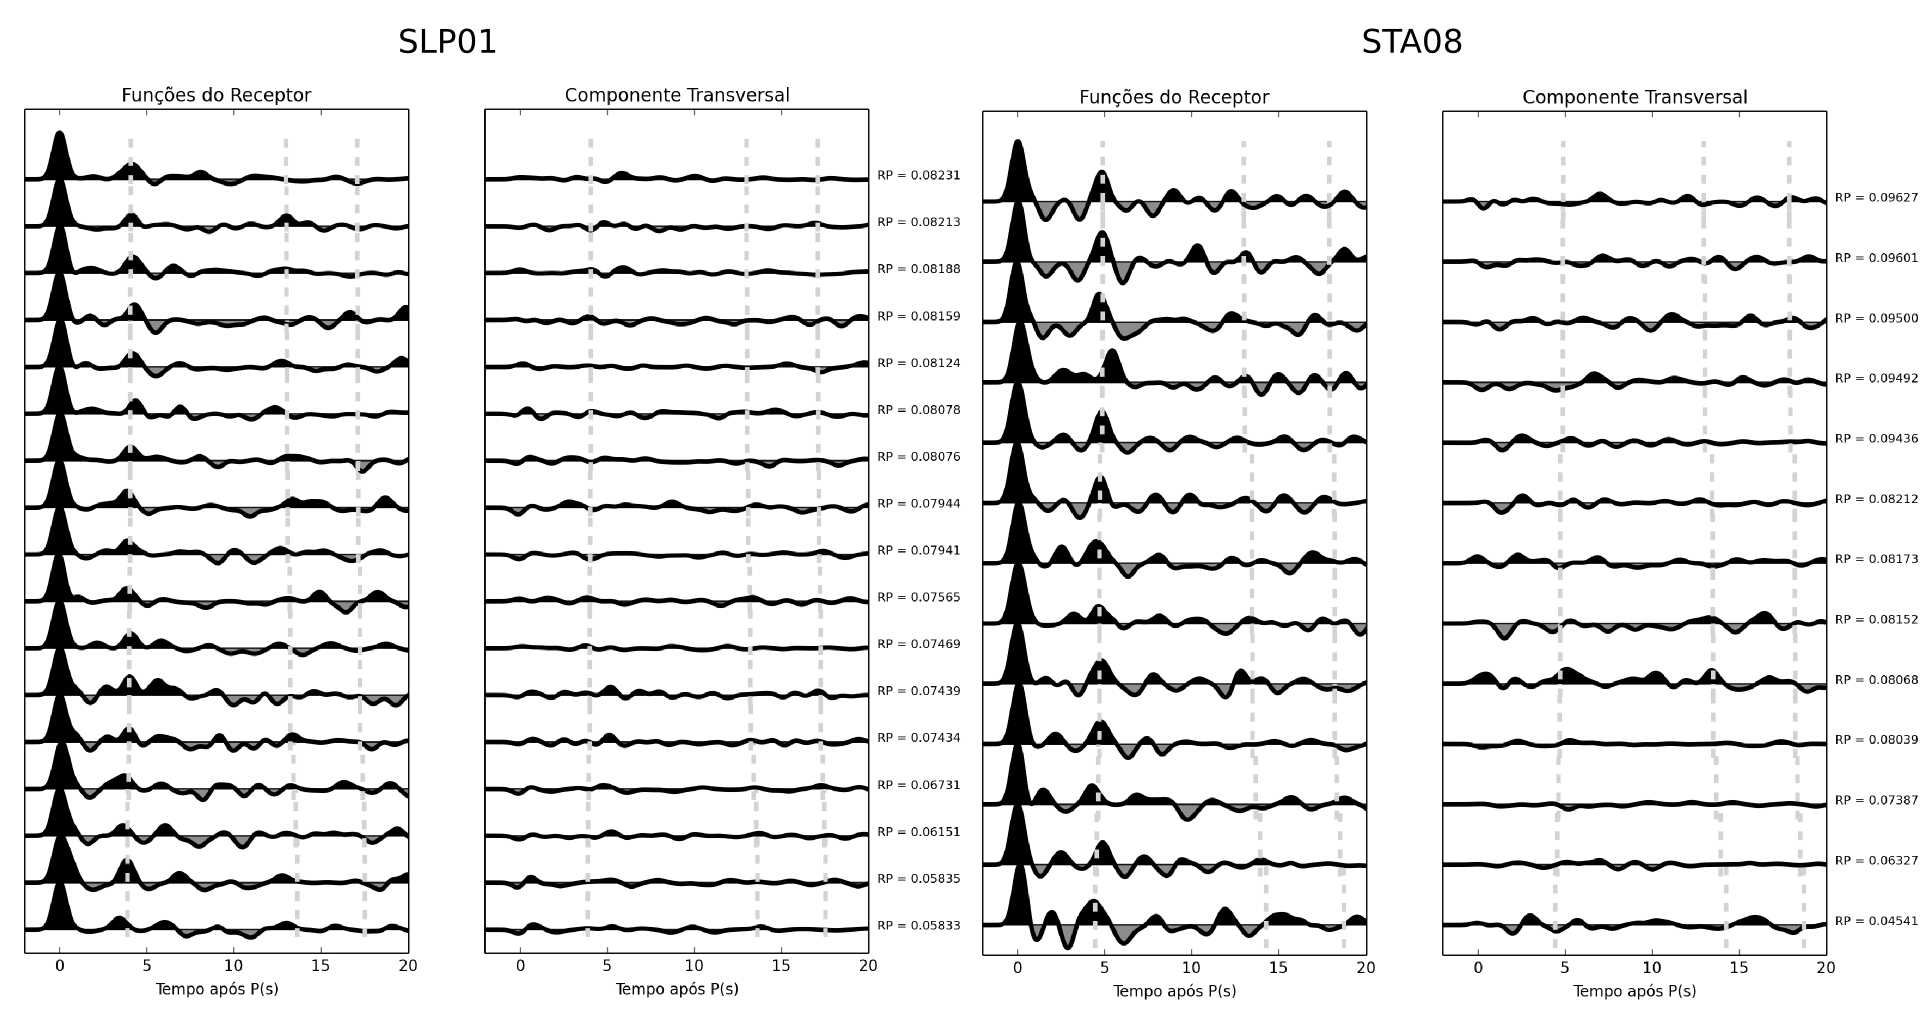
\includegraphics[scale=0.16]{RF_SLP01_STA08.png}
\caption[Exemplos de Funções do Receptor e da Componente Transversal para as estações SLP01(permanete) e STA08(temporária) distribuídas em função do parâmetro do Raio.]{Exemplos de Funções do Receptor e da Componente Transversal para as estações SLP01(permanete) e STA08(temporária) distribuídas em função do parâmetro do Raio. O primeiro pico significa a chegada da onda $P$ direta. Já o segundo a conversão da onda $P$ em $S$ em Moho. As outras múltiplas geradas em Moho não são observáveis. A linha pontilhada simboliza os tempos de chegada teóricos calculados segundo o modelo de \cite{kennet_iaspei_1991}.}
\label{RF_SLP01_STA08}
\end{figure}

DISCUSSÕES SOBRE A COMPONENTE TANGENCIAL - SAVAGE(1998)

Com as Funções do Receptor calculadas, utilizou-se a método desenvolvido por \cite{Zhu_Kanamori_2000} para calcular a profundidade de Moho e a razão $v_{p}/v_{s}$ nas estações sismográficas. Os resultados gerados estão descritos na tabela \ref{tabela1}. Para uma melhor visualização dos resultados gerados, as profundidades de Moho foram interpoladas. Para melhorar a distribuição espacial das profundidades de Moho adicionou-se dados de \cite{Assumpcao_Brazil_2013}. O mapa da interpolação pode ser visto na Figura \ref{Interpolacao}. Nota-se na Figura \ref{Interpolacao} que a discontinuidade de Moho estimada é maior no interior do continente do que na região costeira, corroborando com os dados de \cite{Assumpcao_America_2013}, \citep{Assumpcao_Brazil_2013} e \cite{van_der_meijde_gravity_2013} . 

\begin{figure}[!ht]
\centering
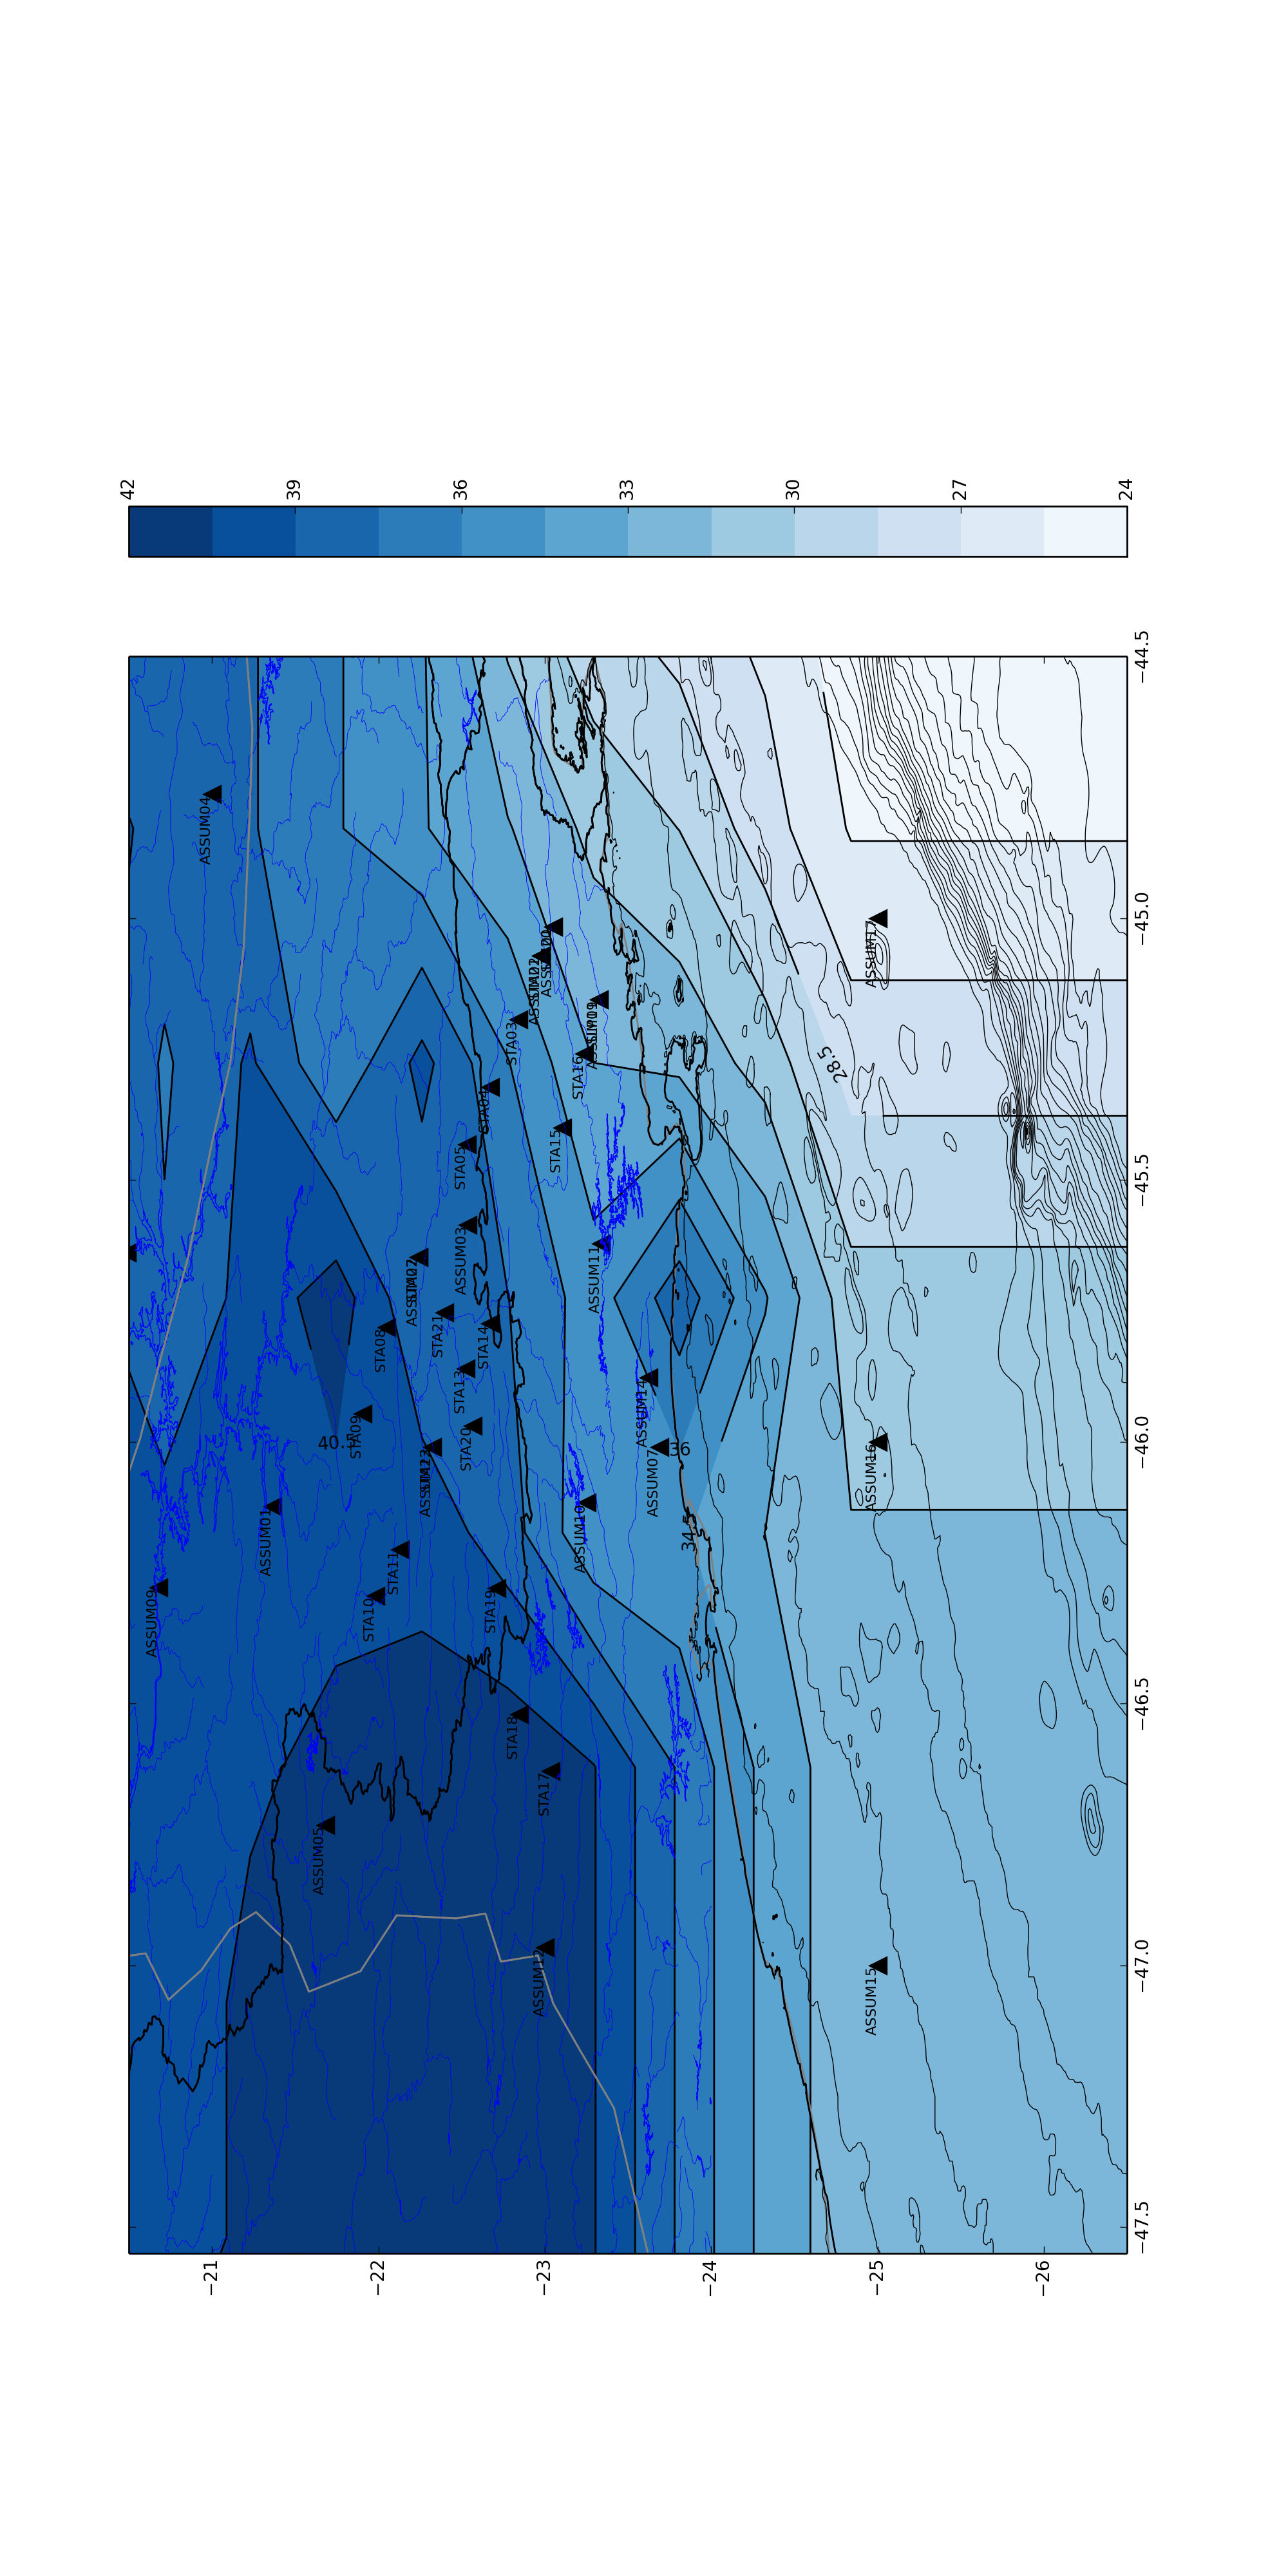
\includegraphics[scale=0.20]{Interpolacao_Linear.png}
\caption{Mapa da espessura crustal da Faixa Ribeira. Os triângulos representam as estações sismograficas.}
\label{Interpolacao}
\end{figure}

As incertezas na medidas, mostradas na Tabela \ref{tabela1}, estão diretamente ligadas a quantidade e qualidade das Funções do Receptor. A seleção das melhores Funções do Receptor é um fase importante, pois a qualidade da Função do Receptor é prepoderante sobre a quantidade. A imprecisão associada a cada um dos parâmetros obtidos pelo método de \cite{Zhu_Kanamori_2000} é estimada pelo método "\textit{bootstrap}", desenvolvido por \cite{efron_statistical_1991}. Neste trabalho utilizou 200  subconjuntos para se fazer a estimativa das incertezas associadas ao  cálculo da profunidade de Moho e da razão $v_{p}/v_{s}$.

\begin{figure}[!ht]
\centering
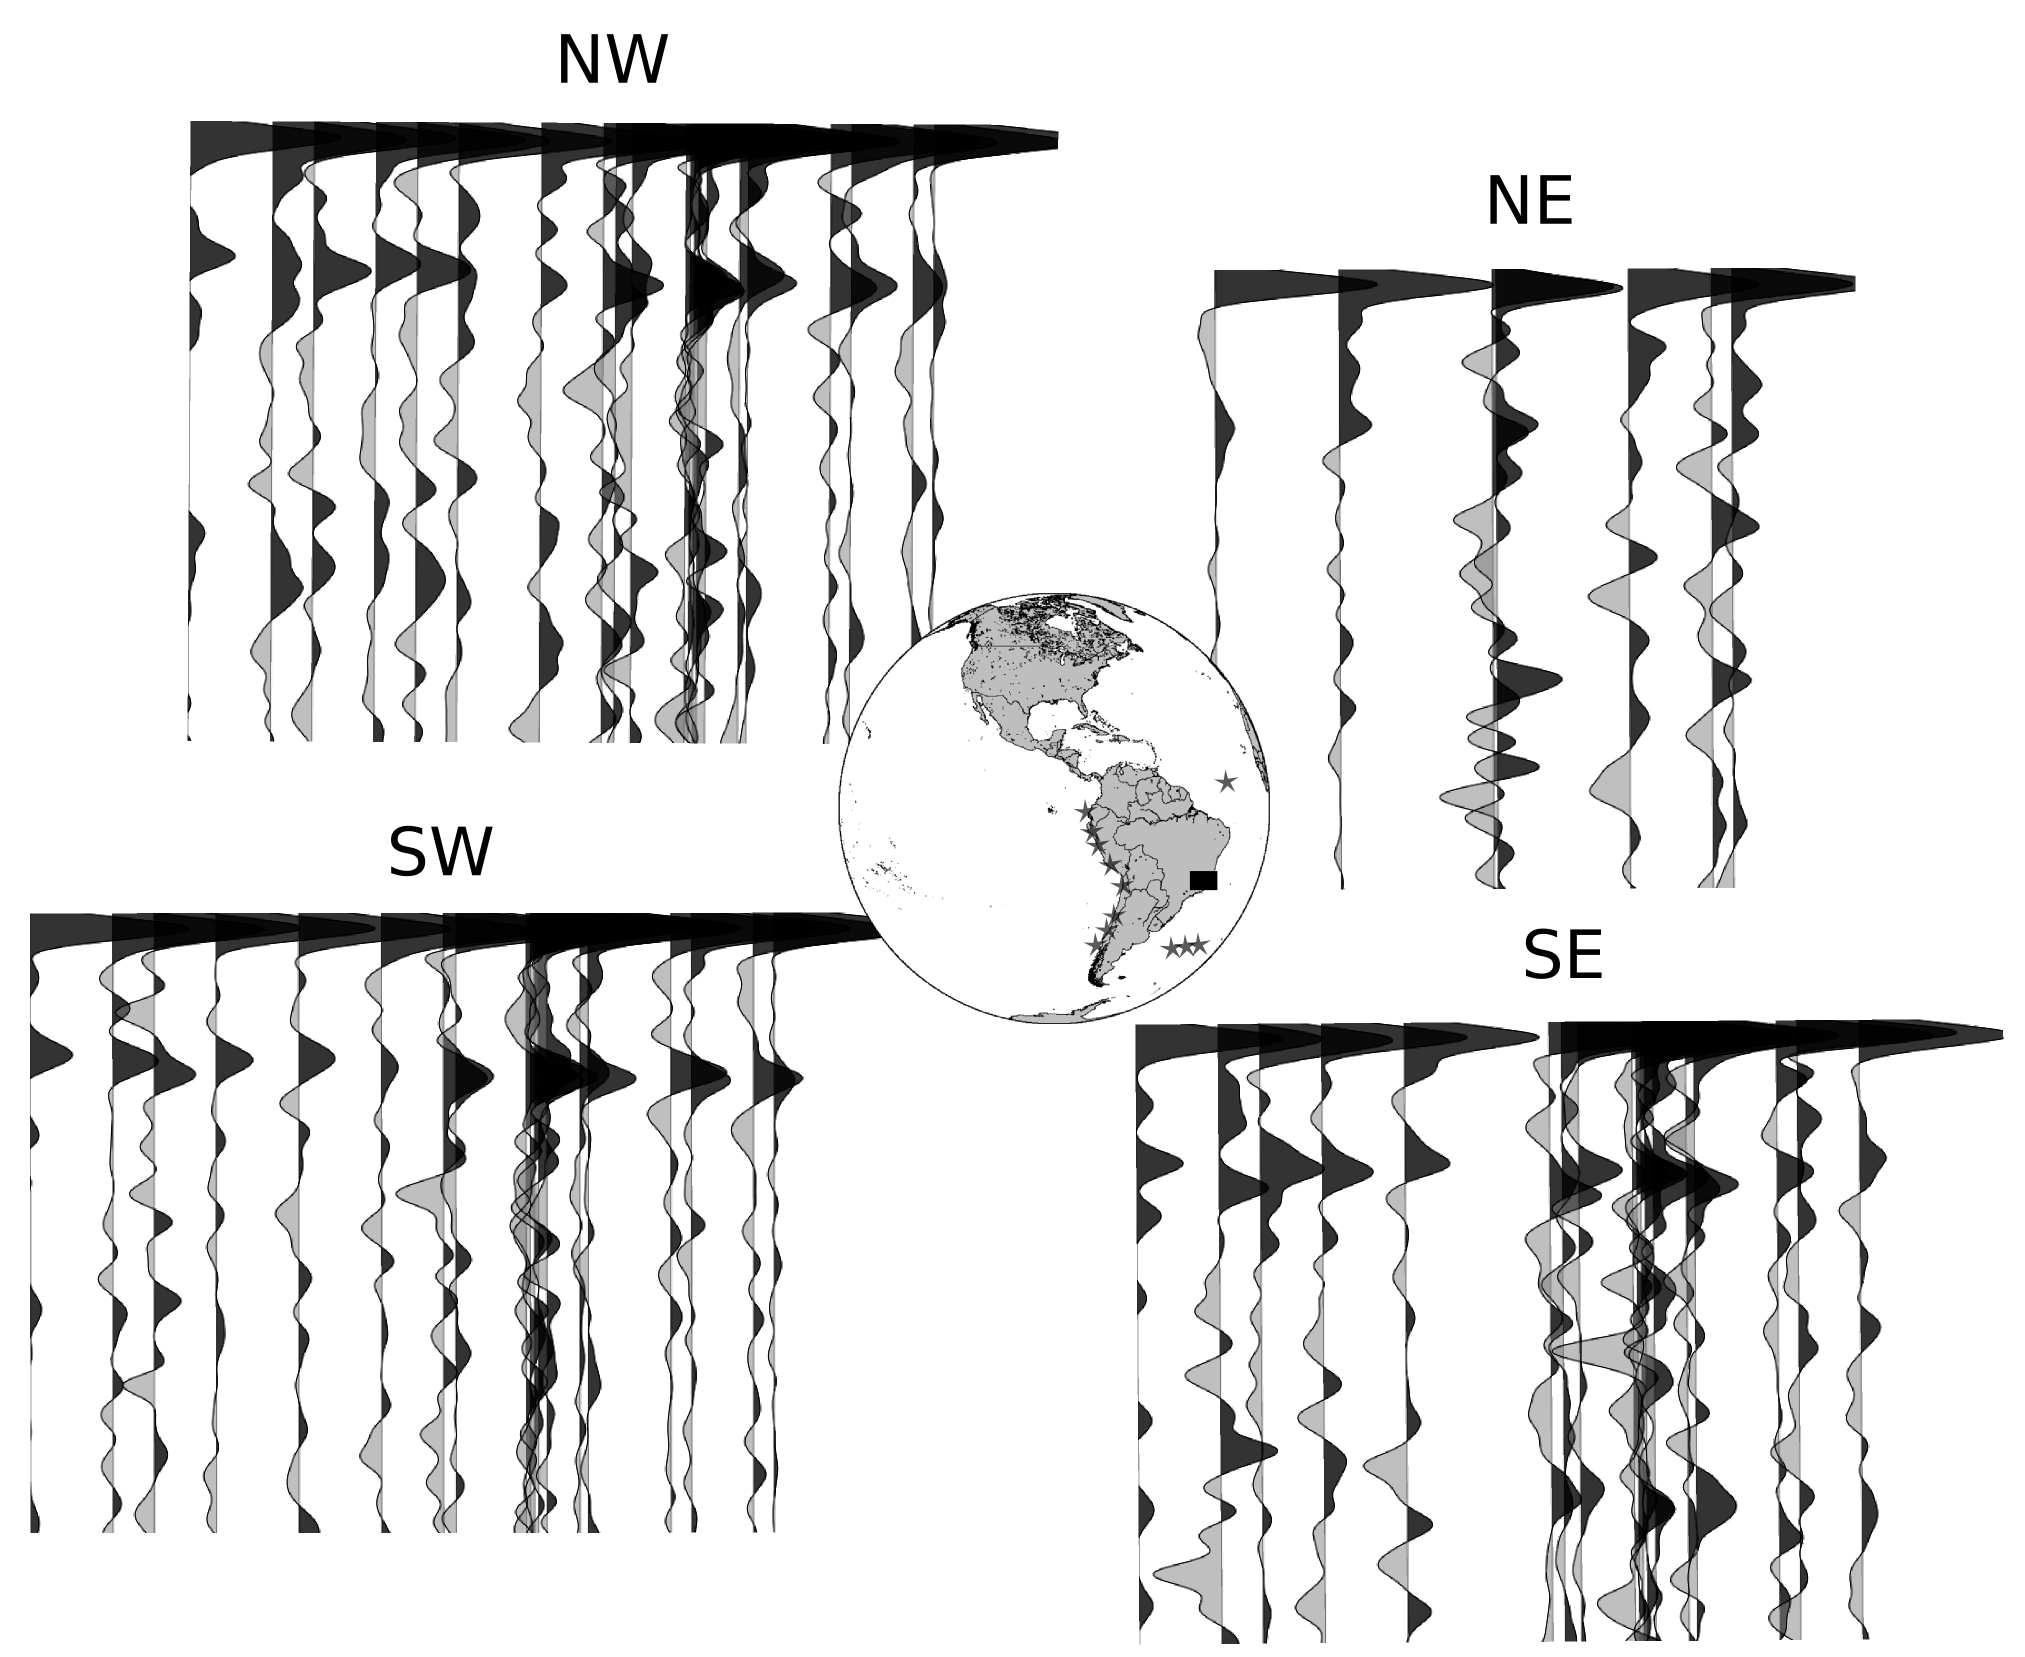
\includegraphics[scale=0.5]{RF_azimute.png}
\caption{}
\label{RF_perfil_NW}
\end{figure}


%Identfica-se sinais precursores a Moho, por volta de 2 a 4 segundos, que variam ao longo do perfil. Estes sinais podem ser relacionados com uma interface com um alto contraste de propriedade fisica. O pulso negativo antes de 5 segundos indica, segundo as modelagens propostas na Figura \ref{modelagem}, uma camada com baixa velocidade.
